% AEES method overview schematic.
%
% Pure schematic, no input data. A three-region block diagram:
%   1. Training loop (left)        : per-step boxes
%   2. Episode controller (right)  : two stacked bandit controllers
%   3. Bridge (center / bottom)    : arm values forward, reward backward
%
% Build (single command; produces a tightly-cropped PDF + PNG):
%   pdflatex -interaction=nonstopmode \
%            -output-directory results/plots/method \
%            scripts/plots/method/aees_overview.tex \
%   && gs -o results/plots/method/aees_overview.cropped.pdf \
%         -sDEVICE=pdfwrite -dUseCropBox \
%         results/plots/method/aees_overview.pdf
%
% The figure is a single tikzpicture; pdflatex emits a one-page PDF sized to
% the figure bounding box (preview / tightpage). The PDF can be included in
% the thesis directly with 
\includegraphics{aees_overview}.
\documentclass{article}

\usepackage[T1]{fontenc}
\usepackage{lmodern}
\usepackage{amsmath}
\usepackage{amssymb}
\usepackage{xcolor}
\usepackage[paperwidth=17.6cm,paperheight=9.4cm,margin=0pt]{geometry}
\usepackage{tikz}
\usetikzlibrary{arrows.meta, positioning, calc, fit, backgrounds}

\pagestyle{empty}
\setlength{\parindent}{0pt}
\setlength{\parskip}{0pt}

% Two-tone palette: cool slate for the training loop, warm sand for the
% bandit controllers. Matches the rest of the thesis schematic aesthetic.
\definecolor{trainfill}{HTML}{DDE6EF}
\definecolor{trainedge}{HTML}{3B5266}
\definecolor{banditfill}{HTML}{F3E2C4}
\definecolor{banditedge}{HTML}{8A6A2B}

\begin{document}
\noindent\hspace*{0.2cm}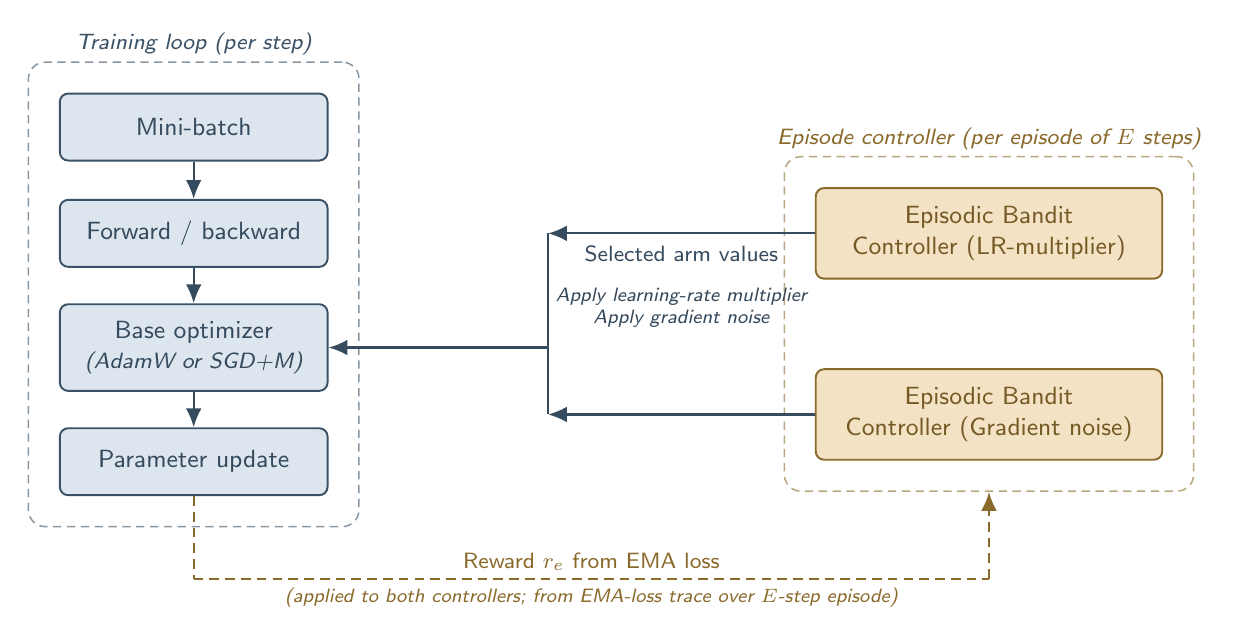
\begin{tikzpicture}[
    font=\sffamily\small,
    >={Latex[length=2.4mm,width=2.0mm]},
    trainbox/.style={
      draw=trainedge, fill=trainfill,
      rounded corners=3pt, line width=0.7pt,
      align=center,
      minimum width=3.4cm, minimum height=0.85cm,
      inner sep=3pt,
      text=trainedge!92!black,
    },
    banditbox/.style={
      draw=banditedge, fill=banditfill,
      rounded corners=3pt, line width=0.7pt,
      align=center,
      minimum width=4.4cm, minimum height=1.15cm,
      inner sep=3pt,
      text=banditedge!85!black,
    },
    flowarrow/.style={->, line width=0.8pt, color=trainedge!92!black},
    bridgearrow/.style={->, line width=0.8pt, color=trainedge!92!black},
    bridgeline/.style={line width=0.8pt, color=trainedge!92!black},
    rewardarrow/.style={->, dashed, line width=0.8pt, color=banditedge,
                        dash pattern=on 3.5pt off 2.2pt},
    rewardline/.style={dashed, line width=0.8pt, color=banditedge,
                       dash pattern=on 3.5pt off 2.2pt},
    regionbox/.style={dashed, rounded corners=6pt, line width=0.55pt,
                      inner sep=11pt,
                      dash pattern=on 3pt off 2pt},
    regionlabel/.style={font=\sffamily\itshape\footnotesize, anchor=south,
                        inner sep=2pt},
    bridgelabel/.style={font=\sffamily\footnotesize,
                        color=trainedge!92!black, align=center, inner sep=1pt},
    bridgesublabel/.style={font=\sffamily\itshape\scriptsize,
                           color=trainedge!88!black, align=center, inner sep=1pt},
    rewardlabel/.style={font=\sffamily\footnotesize,
                        color=banditedge, align=center, inner sep=1pt},
    rewardsublabel/.style={font=\sffamily\itshape\scriptsize,
                           color=banditedge, align=center, inner sep=1pt},
  ]

  % -----------------------------------------------------------
  % Training-loop column (left)
  % -----------------------------------------------------------
  \node[trainbox] (mb)  at (0, 5.55) {Mini-batch};
  \node[trainbox] (fb)  at (0, 4.20) {Forward / backward};
  \node[trainbox, minimum height=1.1cm]
                  (opt) at (0, 2.75) {Base optimizer\\
                                      \footnotesize\itshape(AdamW or SGD+M)};
  \node[trainbox] (pu)  at (0, 1.30) {Parameter update};

  \draw[flowarrow] (mb)  -- (fb);
  \draw[flowarrow] (fb)  -- (opt);
  \draw[flowarrow] (opt) -- (pu);

  % -----------------------------------------------------------
  % Bandit-controller column (right)
  % -----------------------------------------------------------
  \node[banditbox] (blr) at (10.10, 4.20)
                          {Episodic Bandit\\Controller (LR-multiplier)};
  \node[banditbox] (bgn) at (10.10, 1.90)
                          {Episodic Bandit\\Controller (Gradient noise)};

  % -----------------------------------------------------------
  % Region outlines (rendered behind everything)
  % -----------------------------------------------------------
  \begin{scope}[on background layer]
    \node[regionbox, draw=trainedge!60, fit=(mb)(pu)]  (trainregion)  {};
    \node[regionbox, draw=banditedge!60, fit=(blr)(bgn)] (banditregion) {};
  \end{scope}
  \node[regionlabel, color=trainedge] at (trainregion.north)
        {Training loop (per step)};
  \node[regionlabel, color=banditedge] at (banditregion.north)
        {Episode controller (per episode of $E$ steps)};

  % -----------------------------------------------------------
  % Bridge: selected arm values (controllers -> optimizer)
  % -----------------------------------------------------------
  % Vertical rail at the midpoint between the columns.
  \coordinate (rail)    at (4.50, 3.05);
  \coordinate (railtop) at (rail |- blr.west);
  \coordinate (railbot) at (rail |- bgn.west);

  \draw[bridgearrow] (blr.west) -- (railtop);
  \draw[bridgearrow] (bgn.west) -- (railbot);
  \draw[bridgeline]  (railtop)  -- (railbot);

  % Arrow from the rail into the optimizer's right edge: a clean L-shape so
  % the connector stays below the bridge labels and never crosses them.
  \coordinate (railelbow) at (rail |- opt.east);
  \draw[bridgeline]  (rail)     -- (railelbow);
  \draw[bridgearrow] (railelbow) -- (opt.east);

  % Bridge labels (sit in the space between rail and the LR controller,
  % vertically centered in the gap between the two bandit boxes).
  \coordinate (lblanchor) at ($(rail)!0.50!(blr.west)$);
  \node[bridgelabel,    anchor=south] at ($(lblanchor)+(0,0.18)$)
        {Selected arm values};
  \node[bridgesublabel, anchor=north] at ($(lblanchor)+(0,-0.08)$)
        {Apply learning-rate multiplier\\Apply gradient noise};

  % -----------------------------------------------------------
  % Reward: training -> bandit region (terminates on region bottom edge).
  % The horizontal segment sits well below the training region so the two
  % dashed rectangles never appear to share an edge.
  % -----------------------------------------------------------
  \coordinate (rwdcorner1) at ($(pu.south)+(0,-1.05)$);
  \coordinate (rwdcorner2) at (banditregion.south |- rwdcorner1);

  \draw[rewardline]  (pu.south)   -- (rwdcorner1);
  \draw[rewardline]  (rwdcorner1) -- (rwdcorner2);
  \draw[rewardarrow] (rwdcorner2) -- (banditregion.south);

  \coordinate (rwdlbl) at ($(rwdcorner1)!0.5!(rwdcorner2)$);
  \node[rewardlabel,    anchor=south] at ($(rwdlbl)+(0,0.06)$)
        {Reward $r_e$ from EMA loss};
  \node[rewardsublabel, anchor=north] at ($(rwdlbl)+(0,-0.08)$)
        {(applied to both controllers; from EMA-loss trace over $E$-step episode)};

\end{tikzpicture}
\end{document}
